\documentclass[11pt]{article}
\newcommand{\thetitle}{Understanding Systematic Errors Through Modeling of ALMA 
Primary Beams}
\newcommand{\theauthor}{Kara Kundert, Urvashi Rao, Edwin Bergin, Sanjay 
Bhatnager}
\newcommand{\theauthorsemail}{kkundert@umich.edu, rurvashi@nrao.edu, 
ebergin@umich.edu, sbhatnag@nrao.edu}
\newcommand{\thedate}{September 1, 2015}
% the following controls some aspects of how the text is displayed on the page
\setlength{\textwidth}{6.5in}
\setlength{\textheight}{8.0in}
\setlength{\oddsidemargin}{0in}

% set up the page headers and footers
\usepackage{fancyhdr}
    \pagestyle{fancy}
    \lhead{\sffamily\slshape\small\thetitle}
    \rhead{}
    \cfoot{\sffamily\slshape\small\thepage}

% support display of graphics
\usepackage{graphicx}

% gain control over floating objects
\usepackage{float}

% gain control over multiple related figures
\usepackage{subfig}

% import library of technical symbols
\usepackage{amsmath,amssymb,latexsym}

% import bibliography tools
\usepackage{cite}

% the following control some aspects of how paragraphs are displayed
\parindent=0pt
\parskip=2ex

\begin{document}
% print the title in san-serif font, in bold, in huge characters
\title{
    \sffamily\bfseries\huge
    \thetitle \\
}
% print the author in san-serif font
\author{
    \sffamily\theauthor \\
    \sffamily\theauthorsemail \\
}
\date{\thedate}
\maketitle
\sloppy

\section{Abstract}

Many aspects of the ALMA instrument are still unknown due to its young age.
One such aspect is the true nature of the primary beam of each baseline, and
how changes to the individual primary beams affect astronomical
observations. This project aims to create a more thorough
understanding of the strengths and weaknesses of ALMA through realistic
modeling of the primary beams and simulated observations. Results are
quantified by examining the dynamic range of each observation, along with the
ability to reconstruct the amplitude of the test sources. These tests
concluded that the largest contributors to error were changes in antenna
size (i.e. an observation using both the 7m and 12m arrays) and pointing
offsets, followed by offsets in the aperture illumination. In observations of 
large extended sources, deconvolution errors dominated the reconstructed images 
and the individual primary beam errors were indistinguishable from each other.

\section{Introduction}

Radio interferometry has been a key innovation in the field of modern 
astronomy~\cite{swenson-mathur}.  The ability to sync together the observations 
of many separate antennas, along with dramatically improved bandwidths and 
backend technology, has led to incredible observational sensitivities and 
precision in resolution.  However, as capabilities of interferometers and 
digital backends continue to grow, new challenges have come to light. As 
overall noise in processed images continues to diminish with lower system 
temperatures and improved data reduction algorithms, new sources of error have 
begun to surface. 

Systematic errors in instrumentation and digital data pipelines are some of the 
greatest obstacles that astronomers face in the modern field. Over time, the 
nature of these errors has radically changed. As the digital age has blossomed, 
every aspect of the backend of an interferometric array has seen incredible 
improvements - from plummeting system temperatures to ballooning bandwidth 
capabilities. These improvements have led to the lowest systematic levels of 
noise ever seen in radio astronomy.  As the technology used to create the 
digital backends of observatories continues to see astounding rates of 
progress, new sources of systematic errors that were previously easily ignored 
are beginning to make their way above the ever falling noise floor. These newly 
unearthed sources of error have yet to be characterized and thoroughly 
understood, making them an especially treacherous threat for the astronomers 
using the observatories.

Though there are many factors contributing to each image, one that remains 
relatively unexplored is that of how the primary beam affects both the data 
collected and the final images produced~\cite{corder}. As primary beams are 
related to the baseline apertures through a simple Fourier transform, the 
primary beam of each baseline offers a unique insight into the relative state 
of the antennas in an array. Without a thorough understanding of the health of 
the individual antennas and their relationships to each other while performing 
observations, new errors can proliferate into the images through incorrect 
calibration of the primary beam in the imaging process. Such errors include but 
are not limited to the hiding of low-amplitude sources in the side lobes of 
brighter sources and an overall increase in the noise floor of an observation.

Intrinsically, there are two questions to be answered about these new sources 
of error. What effects are they imparting on astronomical observations, and how 
can those effects be corrected? The work done on this simulation aims primarily 
to answer the first question. By creating a thorough and realistic model of 
ALMA, the simulation can observe the propagation of errors generated by 
selectively introducing perturbations to the primary beams. From this 
knowledge, software can be developed to target the largest sources of error in 
data analysis.

\section{Background}

In the case of the ALMA and similar instruments, the visibility function is 
observed and converted into images
via a Fourier transform. As the interferometer is neither infinite in size nor 
sampling at every point in space, each visibility measurement becomes a 
discrete linear weighted sum of a range of spatial frequencies which are 
determined by the geometry of the instrument. The interferometer works by 
combining a set of
antennas into a set of baseline apertures, $A$, which is a Fourier pair with
the primary beam, $PB$. In dealing with the image, the estimated
primary beam of a given observation can be factored out in the final stages of
data corrections and reduction, or used to correct the image using 
A-projection~\cite{bhatnager}.  In order to be able to make this correction, 
the primary beam must be known.
The better the estimated beam matches the true beam from the instrument,
the better the corrections on the data will be. The main question this 
simulation is that of how much uncorrected changes in the primary beams of ALMA 
affect the final images produced using standard CLEAN methods.

In its most basic form, for one timestep, baseline, and polarization, we get 
this Fourier pair of equations:

\begin{equation}
    \label{eq:vis}
    V_{obs} = V_{true} * A
\end{equation}
\begin{equation}
    \label{eq:im}
    I_{obs} = I_{true} \times PB
\end{equation}

where $V_{obs}$ is the observed visibility, $V_{true}$ is the true visibility, 
$I_{obs}$ is the observed image, and $I_{true}$ is the true image. Note that 
$*$ denotes the convolution function, and $\times$ is multiplication.  For a 
source defined on the celestial sphere, the Fourier relationship between the 
visibility function and the image is given by ~\eqref{eq:van-cittert}, commonly 
known as the van-Cittert-Zernike theorem~\cite{tms}.

\begin{equation}
    \label{eq:van-cittert}
    V(u,v) = \iint I(l,m) e^{-2 \pi i (ul + vm))} dl dm
\end{equation}

Each visibility measurement in this case is an integral of the true visibility 
plane over the baseline aperture function. In this simplified case of a 
snapshot on one polarization over one baseline, we can hypothetically make this 
Fourier transform in order to factor the primary beam out of the observed image 
to regain the true image. This is the mathematical foundation of the 
simulation.

\subsection{The ALMA Observatory}

In the case of ALMA, the array is still in its early science phase, so some 
parameters are bound to change as the remaining components of the instrument 
gradually come online. In its final design, ALMA will consist of a 12-m array, 
a compact 7-m array, and 4 12-m antennas for single dish (or Total Power) 
observations.  The 7-m and total power arrays - with their overall shorter 
baselines - aims to fill the hole in UV coverage typically seen in radio 
interferometers. Located on the Chajnantor plain of the Chilean Andes, the full 
combined array will have several configurations with an absolute maximum 
baseline of up to approximately 16 km. It will be capable of observing from 
31-950 GHz with full linear polarization (X, Y)~\cite{alma-tech-handbook}.

However, ALMA is not yet fully finished. In Early Science Cycle 
2 - which the simulation aims to model - the array has the following 
specifications: 34 12-m antennas of three separate designs, along with the 
Atacama Compact Array (ACA), which consists of nine identical 7-m 
dishes~\cite{cycle-2-capabilities}. There are also two 12-m antennas in the 
Total Power Array, used to make single dish observations in order to fill the 
central hole in the u-v place. Each antenna is equipped with receivers to 
observe at bands 3, 4, 6, 7, 8, and 9, which corresponds to wavelengths of 
about 3.1, 2.1, 1.3, 0.87, 0.74, and 0.44 mm. There are many configurations of 
the array, with maximum baselines ranging from approximately 160 m to 1.5 km, 
though the maximum baseline for bands 8 and 9 is approximately 1 km.

One fact is evidently clear - ALMA is the foremost leader in interferometric 
imaging at any wavelength. As image fidelity is most strictly limited by the 
number and coverage of samples in the u-v plane~\cite{wright}, the sheer number 
of antennas along with the variation in baseline spacings gives ALMA superior 
imaging capabilities to any other modern interferometer currently online. This 
incredible ability means that errors generated by systematic errors in primary 
beam analysis will be quick to limit the imaging capabilities of ALMA.

\subsection{The Model}

This project aims to model a realistic array, with as many of the known 
problems of the ALMA primary beam as we know how to replicate computationally.  
As such, the simulation does the calculations shown in Eqs.~\eqref{eq:vis} 
and~\eqref{eq:im} for a set of mutually unique aperture models over a series of 
time steps. As time progresses in the simulation, so does the relative geometry 
of the array to the celestial sphere.

The simulation itself is simple in concept. A numerical interferometer is 
constructed by generating a set of apertures in an array. The shape and 
placement of the array are fed into the simulation. Consideration must be given 
to matching the geometry of the array with the size of the images desired and 
the size of a pixel, such that Nyquist sampling is achieved. The simulation is 
designed to be a test of the capabilities of ALMA in Cycle 2 of its early 
science testing. Therefore, the unperturbed numerical interferometer which acts 
as the control case of the simulation has 34 identical apertures, taking data 
in receiver band 3. The maximum baseline is approximately 800 m.
The apertures studied were complex apertures constructed from holography 
measurements of the actual ALMA antennas, modified to remove support leg 
diffraction effects. A representative sample of these apertures is shown in
Figure~\ref{fig:apertures}. These were chosen as they were the closest to 
reality as could be attained with current available models, including the 
illumination offset features. These apertures also include imaginary structure, 
which opens up the possibility for future investigation into how the
errors from beam perturbations carry through the Stokes polarization planes.

\begin{figure}
    \centering
    \subfloat[DA Measured Aperture - Real]{
        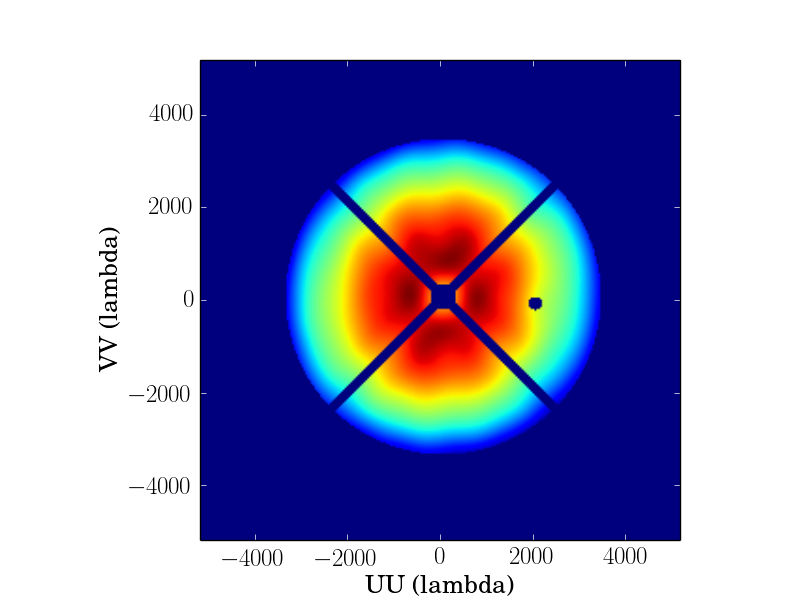
\includegraphics[height=2.2in]{images/fits/aperture_real.png}
        \label{fig:da-real}
    }
    \quad
    \subfloat[DA Measured Aperture - Imaginary]{
        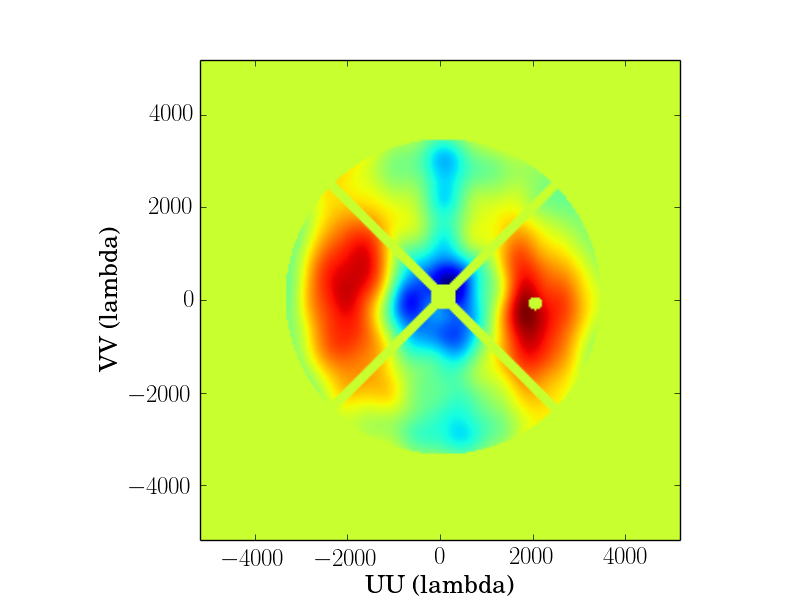
\includegraphics[height=2.2in]{images/fits/aperture_imag.png}
        \label{fig:da-imag}
    }
    \caption{
        A typical example of the real and imaginary components of a 12m DA-type 
        antenna. Asymmetry around the support legs can be observed - this is 
        caused by the illumination offsets from the secondary reflector. While 
        the perturbation in this case is small, the offsets can be very      
        extreme.
     }
    \label{fig:apertures}
\end{figure}

In all tests, the apertures begin without any perturbations - just a flat disk 
with support arms. The perfect aperture is then perturbed to demonstrate 
problems that ALMA is known to have, such as pointing offsets,
noise-like variations on the aperture surface, variations in the illumination 
on the primary reflector, and differences in antenna size to model an 
observation done with the main and compact ALMA arrays. This addresses the 
biggest reality of all arrays - the fact that each antenna is imperfectly 
unique, and in many ways can not be equated with its neighbors in the array.
Time-dependence of the sky was ignored during the simulation, as parallactic 
angle rotation calculations were too computationally expensive to include, and 
was found to be a small effect in generating excess noise in 
images~\ref{tab:rms-10ants}.  Polarization was also largely ignored for the 
sake of time.

By convolving the perturbed apertures, baseline aperture functions are 
calculated for each pair of antennas, the Fourier transform of which gives the 
primary beam of that baseline. This primary beam is multiplied by the true sky 
image, baseline per baseline. Visibilities were calculated from the perturbed 
data to produce a simulated data set. The standard MS-CLEAN task is then run on 
these images of the ``observed sky". The off-source rms-level of the image is 
saved to disk.  Image fidelity is also tested by finding the amplitude of the 
cleaned source divided by the normalized amplitude value of the CASA model 
primary beam at that point.  This test was done to see how closely the primary 
beams need to match in order to get desired fidelity in image reconstruction.

\begin{figure}
    \centering
    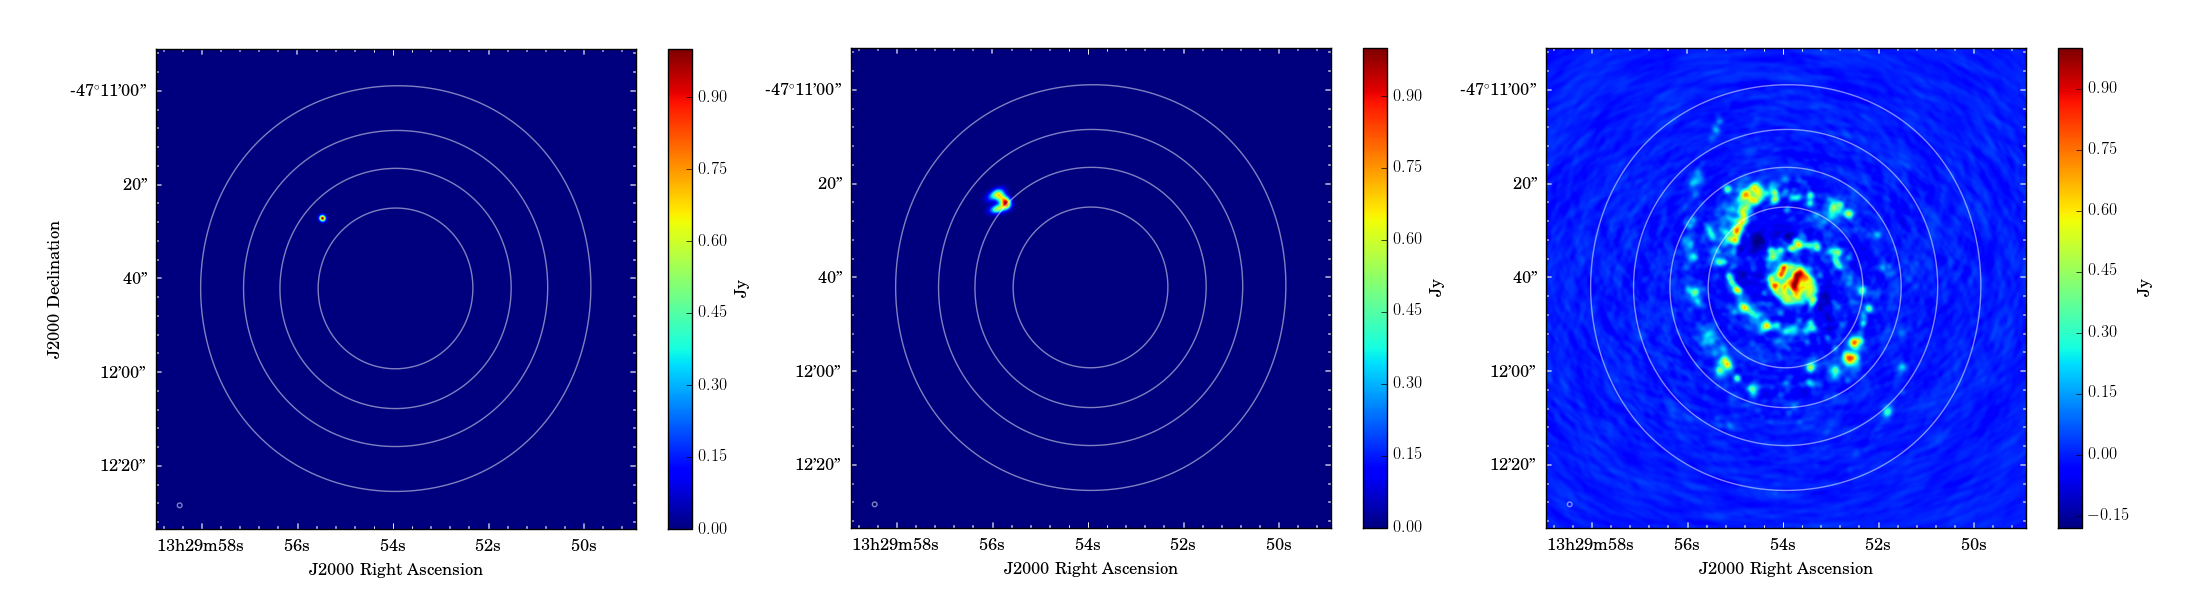
\includegraphics[width=6.5in]{images/fits/all-sources.png}
    \caption{
        The simulated sources used for each test. From left to right, there is 
        the point source, the small extended source, and the large extended 
        source. The smaller sources are offset from the center of the image in 
        order to introduce primary beam effects to the image, as a small 
        centered source will not experience primary beam related perturbations.  
       }
    \label{fig:sources}
\end{figure}

The parameters used for testing were chosen in an effort to minimize testing
time while still getting useful results. As such, the simulation was run
with 34 antennas with 40 snapshots over a 2 hour observation. The uv-coverage
and antenna placement can be seen in Figure~\ref{fig:params}. Three main tests
were run, a 1 Jy point source pointed slightly off-center, a small extended 
source (to emulate a protoplanetary disk or small cloud), and a large extended 
source to fill the whole primary beam, as can be seen in 
Fig.~\ref{fig:sources}.  The source in the point source test was
located at approximate the 75$\%$ power point in the main lobe of an 
unperturbed primary beam. The small extended source was centered at 
approximately the 60$\%$ power level of the main lobe of the unperturbed 
primary beam. The large extended source was centered. \footnote{The small 
 sources were placed off-center in order to observe the effects of primary beam 
 corrections. A point source or small source that is perfectly or nearly 
 perfectly centered in the beam would anticipate very small corrections from 
the primary beam, as it would be located at nearly maximum power.  Primary beam 
correction errors are generated in the lower-power regions and side lobes of 
the image.}

\begin{figure}
    \centering
    \subfloat[Test Antenna Locations]{
        \includegraphics[height=2.2in]{results/new_ants.png}
        \label{fig:locs}
    }
    \quad
    \subfloat[Test UV-Coverage]{
        \includegraphics[height=2.2in]{results/new_uv.png}
        \label{fig:uvcoverage}
    }
    \caption{
        The locations of the 34 antenna array used in all simulations in the
        experiment, and the uv-coverage generated from each observation. A
        hole in the center of the uv-field is clearly seen, as the compact 
        array geometry was not included in the simulation.
    }
    \label{fig:params}
\end{figure}

\begin{figure}
    \centering
    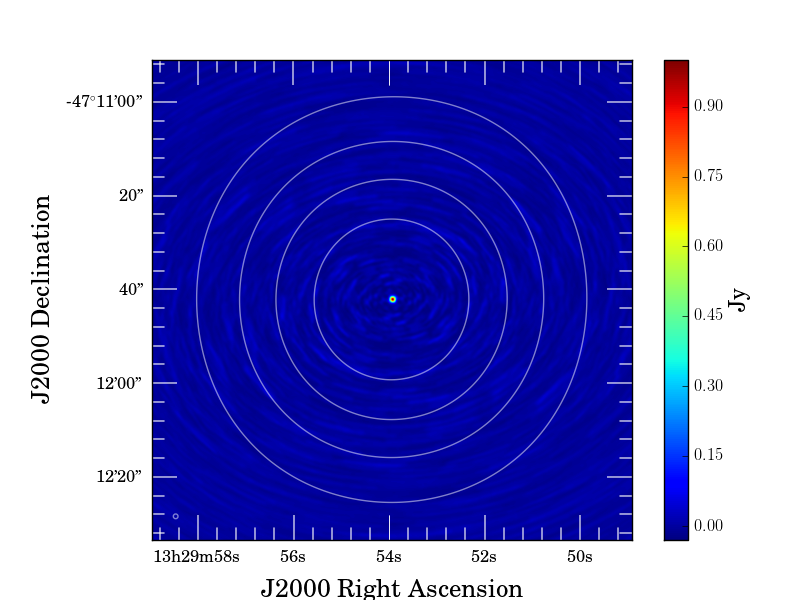
\includegraphics[height=2.2in]{images/fits/psf.png}
    \caption{
        The point-spread function (PSF) of the synthesized beam used in all 
        tests.  Tests were run with an array of 34 antennas, observing 40 
        snapshots over the course of 2 hours.
    }
    \label{fig:psf}
\end{figure}

Future testing hopes to investigate the benefits of A-projection in image 
correction. A-projection uses a model of the aperture in the initial steps of 
imaging and deconvolution in order to remove its effects from the final image.  
The idea goes that the baseline apertures $A$ have contributed various effects 
into the visibilities as they are observed, as described in~\eqref{eq:vis}. In 
order to remove those effects, the observed visibilities must be convolved with 
the inverse of the baseline aperture function $A^{-1}$, as seen 
in~\eqref{eq:a-proj}. The baseline aperture and its inverse will then form a 
unity matrix, returning the true visibilities, which can be Fourier transformed 
into the true image~\cite{bhatnager}.

\begin{equation}
    \label{eq:a-proj}
    V_{true} = A^{-1} * V_{obs}
\end{equation}
\begin{equation}
    \label{eq:a-inv}
    A^{-1} = \frac{A^{\dagger}}{AA^{\dagger}}
\end{equation}

This process takes place during the regridding of the visibilities, so that 
$A^{-1}$ replaces the weighting function that evenly samples the u-v plane.  
However, $AA^{\dagger}$ may contain zero valued components. As such, division 
by $AA{\dagger}$ is an extremely dangerous computation to make, as it has the 
potential to fill the u-v plane with divide-by-zero errors and create an 
entirely erroneous image. Instead, the Fourier transform relationship between 
the aperture and the primary beam is used to rewrite~\eqref{eq:a-proj} and 
\eqref{eq:a-inv} as

\begin{equation}
    \label{eq:a-proj-cor}
    V_{true} = A^{\dagger} * V_{obs}
\end{equation}
\begin{equation}
    \label{eq:imcor}
    PB^2 \overset{\mathcal{F}}{\rightleftharpoons} AA^{\dagger}
\end{equation}

$PB^2$ is then factored out of the final image, minimizing the divide-by-zero 
errors while maintaining the integrity of the A-projection relationship. This 
method allows for a great deal of instrumental image correction prior to 
actually entering the image domain, assuming an accurate model of the aperture 
functions $A$ is used.

\section{Results}

The strongest effects in the simulation were found to be
variation in antenna size and uncorrected pointing offsets, with dynamic range 
limited to less than 1000 in the test case of a single 2 hour observation of a 
1 Jy point source. The next largest effects were illumination offsets and 
  corrected pointing offsets, with dynamic ranges limited to around 10,000.  
  Preliminary testing done in 2013 indicated that other varieties of primary 
  beam perturbations, e.g.  beam rotation, ellipticity, combination of the 
  three kinds of 12m antennas, were relatively minor effects, with dynamic 
  ranges at the $10^5$ level or higher for a single point source observation.  
  Results from the small extended source case indicate generally the same trend 
  in the hierarchy of perturbation of data, though at slightly higher noise 
  levels in all cases.  Results from the large extended source are almost 
  entirely flat, indicating that deconvolution errors are dominating over the 
  problems in the primary beam.

\begin{figure}
    \centering
    \subfloat[No Perturbation]{
        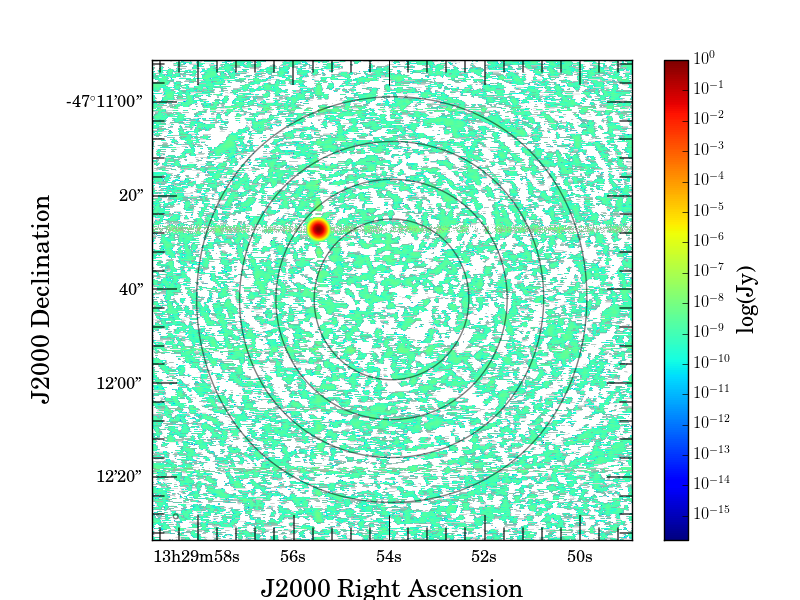
\includegraphics[height=2.2in]{images/fits/no_perturbation_point.png}
        \label{fig:no_perturbation}
    }
    \quad
    \subfloat[Illumination Offset]{
        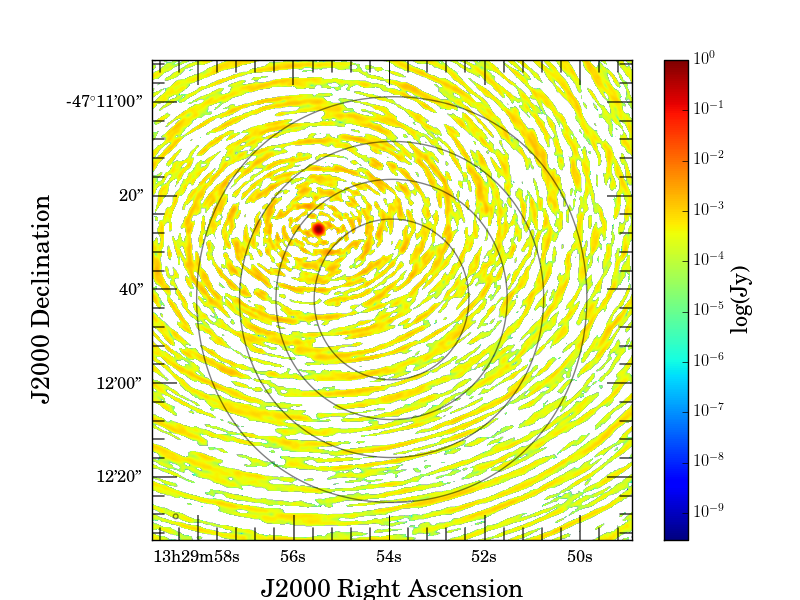
\includegraphics[height=2.2in]{images/fits/illum_offset.png}
        \label{fig:illum_offset}
    }
    \quad
    \subfloat[Corrected Pointing Offsets]{
        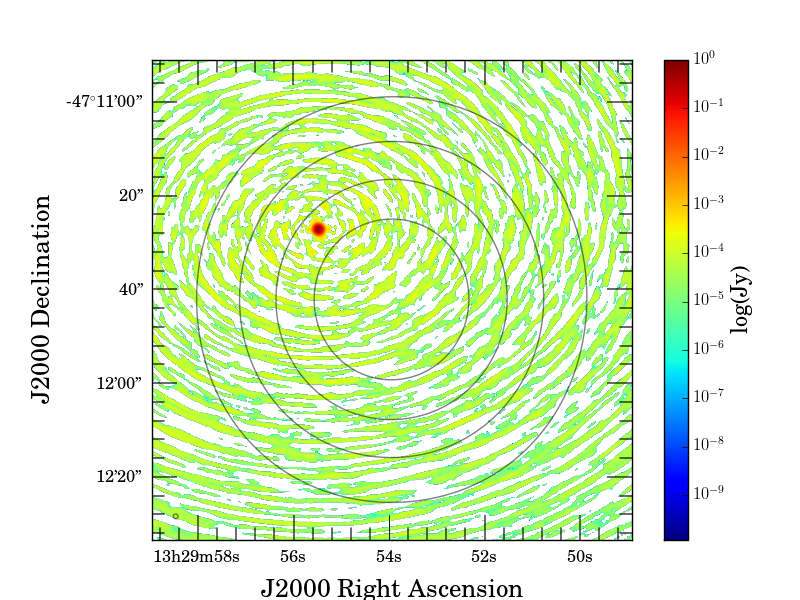
\includegraphics[height=2.2in]{images/fits/pointing_cor_point.png}
        \label{fig:pointing_cor}
    }
    \quad
    \subfloat[Uncorrected Pointing Offsets]{
        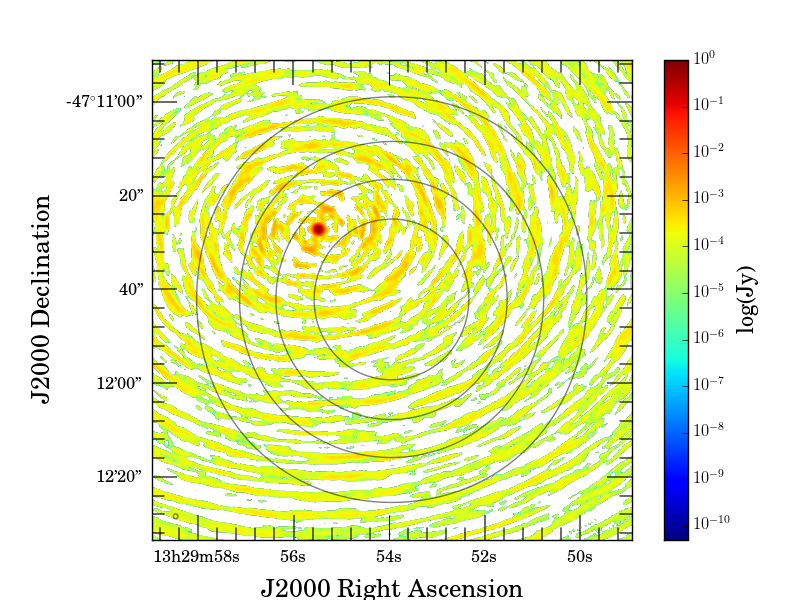
\includegraphics[height=2.2in]{images/fits/pointing_point.png}
        \label{fig:pointing}
    }
    \quad
    \subfloat[Antenna Size Difference]{
        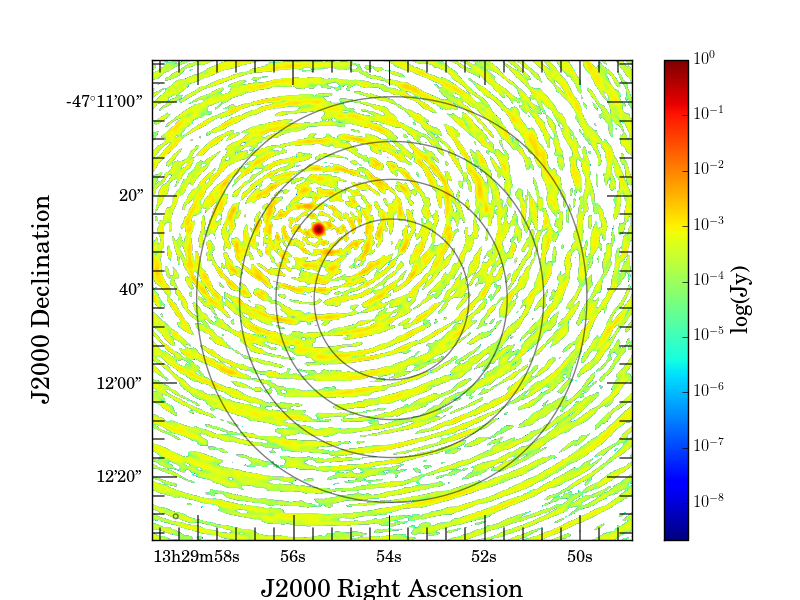
\includegraphics[height=2.2in]{images/fits/size_diff.png}
        \label{fig:size_diff}
    }
    \quad
    \subfloat[All Effects]{
        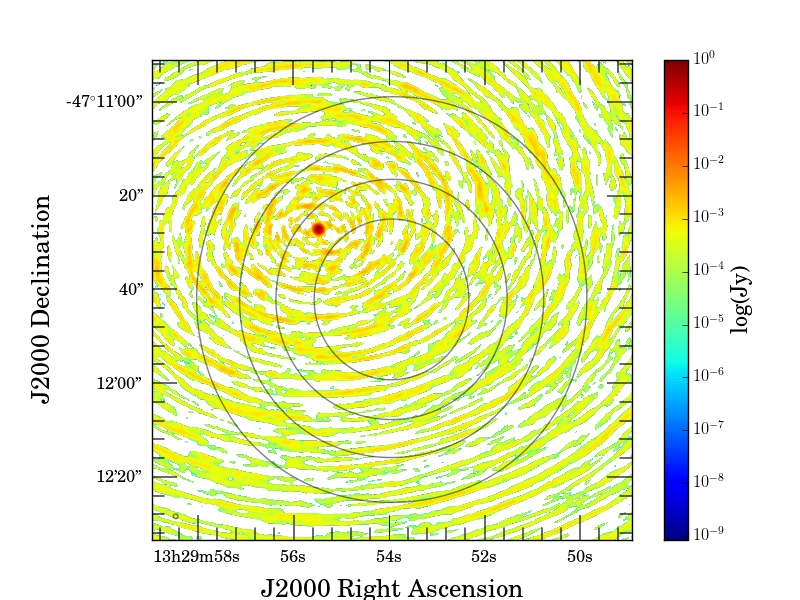
\includegraphics[height=2.2in]{images/fits/all_effects.png}
        \label{fig:all_effects}
    }
    \caption{
        These images show the progression in overall noise as related to the 
        perturbing effects. As noted, uncorrected pointing offsets and using 
        antennas of different sizes are especially immediate concerns, as they 
        lead to dramatic overall increases in noise. All images were saturated 
        to the same level in order to make the background noise visible.
    }
    \label{fig:perturbations}
\end{figure}

The largest perturbation effect came from changing the antenna sizes, with 
inverse dynamic ranges around $ 3.3 \times 10^{-3}$ in the single point source 
test and $5.7 \times 10^{-3}$ in the small extended source test. This kind of 
effect would be generated by using the ALMA 7m and 12m arrays in conjunction 
with each other, with the small baselines of the 7m array filling in the center 
of the uv-coverage plane. There are already computational solutions available 
to astronomers in the CLEAN package that can be used to ameliorate this effect, 
but they are not standard and must be hand-selected during image reduction.


The second largest effect was that of uncorrected pointing offsets, which
range in value from about 2-4 arcseconds. Simulated observations took place
at 100 GHz, giving the primary beam a FWHM of approximately 45 arcseconds.
At worst, the uncorrected pointing offsets could shift the beam by almost
$10\%$ of its width. Tests for this case gave inverse dynamic ranges of $1.0 
\times 10^{-3}$ for the single point source case, and $9.7 \times 10^{-4}$ in 
the small extended source case.

It is worth noting that the change in primary beam size is inversely 
proportional to the frequency. As such, if the observing frequency doubles, the 
primary beam will half its width. Numbers were also given for ALMA's ability to
self-correct for pointing offsets, which have a maximum of 0.5 arcseconds.
Given an observation at 800 GHz with corrected pointing offsets, expected 
rms-levels would be similar to or worse than the case of an uncorrected 
pointing offset at 100 GHz.

RMS-levels for all 34 antenna tests can be found in Table~\ref{tab:rms-34ants}.  
A set of preliminary tests took place in 2013 to determine which perturbations 
merited more thorough investigation. These tests investigated a much broader 
selection of perturbation effects with less precision - the simulation used an 
array of only 10 antennas and 4 time steps over a simulated two-hour 
observation. Tests were run on point source observations, with one point source 
and one multi-source test per perturbation effect. The inverse dynamic ranges 
for these tests are given in Table~\ref{tab:rms-10ants}.

\section{Conclusions}

Initial results show that understanding the primary beam and how it affects
observations is critical to the science being done at these instruments. The
predominant effects on data stem from changes in the size of the aperture
(from using the 7m and 12m antennas in tandem in observations) and in
pointing offsets, uncorrected and corrected at high frequencies. 

The 7m and 12m arrays are designed to be used together, with the 7m array 
filling in the uv-coverage hole that couldn't be filled with the larger 12m 
dishes. With the effect of combining these antennas leading to rms levels of 
greater than 1 mJy, this is an error that cannot afford to be left uncorrected.  
It is probable that this effect is already being seen in ALMA data. The rise in
noise levels probably stems from the combination of three main kinds of
primary beams: those baselines with two 7m antennas, with two 12m
antennas, and those with a 7m and a 12m antenna. Therefore, a reasonable
correction would be to incorporate three model primary beams in the ALMA data 
pipeline, and to divide out primary beams baseline-by-baseline prior to any 
astronomer specific data reduction. This kind of algorithm is already available 
as a non-standard option in the CLEAN task, so modifying it for use in the ALMA 
pipeline should be relatively straightforward.

The next effect to be concerned about would be the case of uncorrected pointing 
offsets and high frequency corrected pointing offsets.
At low frequencies, ensuring that all observations are done with use of 
pointing correction would certainly help. However, observations above 400 GHz 
are liable to see these same limits even with the help of the pointing guides, 
as pointing offsets have an effect that is relative to the size of the beam. As 
frequency goes up and the beam size shrinks, even a corrected pointing offset 
could have severe consequences on image quality. Given that the offsets are 
inherently random, it's difficult to imagine a correction that could be made 
using software - either as part of the ALMA pipeline or as a CASA-type tool for 
astronomers to use as necessary.  If a method could be devised to correct 
pointing offsets at the time of observation to the 0.01 - 0.05 arcsecond level, 
even the highest frequencies would retain dynamic ranges of 10,000 or higher.

With all other effects having much smaller effects on the
residuals in standard imaging procedures, focus should be directed towards
correcting for these larger effects before they start seriously impeding the
scientific goals of the ALMA instrument. Efforts should also be made to improve 
deconvolution algorithms, in order to improve imaging of extended objects to 
the point that primary beam perturbations can begin to affect the data.

\bibliography{primary-beams}{}
\bibliographystyle{plain}

\begin{table}
    \centering
    \begin{tabular}{|p{8cm}|c|c|}
    \hline
    & Single Source & Multi-Source  \\
    \hline
    7m, 12m & $4.55 \times 10^{-5}$ & $2.86 \times 10^{-4}$ \\
    \hline
    Unperturbed NumPy-Generated & $3.17 \times 10^{-9}$ & $2.99 \times
    10^{-9}$ \\
    \hline
    Parallactic Angle Rotation, NumPy-Generated & $6.74 \times 10^{-7}$ &
    $1.84 \times 10^{-5}$ \\
    \hline
    DA/DV, NumPy-Generated & $3.91 \times 10^{-6}$ & $3.89 \times 10^{-5}$ \\
    \hline
    DA/DV with Parallactic Angle Rotation, NumPy-Generated & $3.99 \times
    10^{-6}$ & $4.23 \times 10^{-5}$ \\
    \hline
    Uncorrected Pointing Offsets, NumPy-Generated & $2.85 \times 10^{-5}$ &
    $6.18 \times 10^{-5}$ \\
    \hline
    Corrected Pointing Offsets, NumPy-Generated & $7.82 \times 10^{-6}$ &
    $1.69 \times 10^{-5}$ \\
    \hline
    Corrected Pointing Offsets with Parallactic Angle Rotation,
    NumPy-Generated & $4.78 \times 10^{-6}$ & $2.74 \times 10^{-5}$ \\
    \hline
    DA/DV with Corrected Pointing Offsets, NumPy-Generated & $5.39 \times
    10^{-6}$ & $5.84 \times 10^{-4}$ \\
    \hline
    Unperturbed, CASA Ray-Traced& $3.19 \times 10^{-9}$ & $3.60 \times
    10^{-9}$ \\
    \hline
    Parallactic Angle Rotation, CASA Ray-Traced & $8.52 \times 10^{-7}$ &
    $1.32 \times 10^{-5}$ \\
    \hline
    DA/DV, CASA Ray-Traced & $3.42 \times 10^{-7}$ & $4.53 \times 10^{-6}$ \\
    \hline
    DA/DV with Parallactic Angle Rotation, CASA Ray-Traced & $8.52 \times
    10^{-7}$ & $1.32 \times 10^{-5}$ \\
    \hline
    Uncorrected Pointing Offsets, CASA Ray-Traced & $2.29 \times 10^{-5}$ &
    $4.81 \times 10^{-5}$ \\
    \hline
    Corrected Pointing Offsets, CASA Ray-Traced & $6.19 \times 10^{-6}$ &
    $1.98 \times 10^{-5}$ \\
    \hline
    Corrected Pointing Offsets with Parallactic Angle Rotation, CASA
    Ray-Traced & $7.28 \times 10^{-6}$ & $2.20 \times 10^{-5}$ \\
    \hline
    DA/DV with Corrected Pointing Offsets, CASA Ray-Traced & $5.32 \times
    10^{-6}$ & $1.54 \times 10^{-5}$ \\
    \hline
    Unperturbed, Measured & $4.47 \times 10^{-9}$ & $7.76 \times
    10^{-9}$ \\
    \hline
    Parallactic Angle Rotation, Measured & $4.05 \times 10^{-6}$ &
    $2.48 \times 10^{-5}$\\
    \hline
    DA/DV, Measured & $3.13 \times 10^{-6}$ & $2.84 \times 10^{-5}$ \\
    \hline
    DA/DV with Parallactic Angle Rotation, Measured & $5.83 \times
    10^{-6}$ & $2.78 \times 10^{-5}$ \\
    \hline
    Uncorrected Pointing Offsets, Measured & $1.27 \times 10^{-5}$
    & $5.90 \times 10^{-5}$ \\
    \hline
    Corrected Pointing Offsets, Measured & $4.70 \times 10^{-6}$ &
    $1.33 \times 10^{-5}$\\
    \hline
    Corrected Pointing Offsets with Parallactic Angle Rotation, Measured & 
    $8.78 \times 10^{-6}$ & $2.93 \times 10^{-5}$ \\
    \hline
    DA/DV with Corrected Pointing Offsets, Measured & $2.49 \times
    10^{-5}$ & $6.28 \times 10^{-5}$ \\
    \hline
    Illumination Offsets, Measured & $8.85 \times
    10^{-5}$ & $2.46 \times 10^{-5}$ \\
    \hline
    \end{tabular}
    \caption{
        Approximate inverse dynamic range levels found in the corrected images 
        of the preliminary runs of the simulation, using 10 antennas and 4 time 
        steps.
    }
    \label{tab:rms-10ants}
\end{table}

\begin{table}
    \centering
    \begin{tabular}{|p{3.5cm}|c|c|c|}
    \hline
    & Point Source & Small Extended Source \linebreak (Off-Center) & Large 
    Extended Source \\
    \hline
    No Perturbation & $6.0 \times 10^{-8}$ & $7.6 \times 10^{-5}$ & 0.013 \\
    \hline
    Corrected Pointing \linebreak Offsets & $2.1 \times 10^{-4}$ & $2.6 \times 
    10^{-4}$ & 0.013 \\
    \hline
    Illumination \linebreak Offsets & $2.8 \times 10^{-4}$ & $4.6 \times 
    10^{-4}$ & 0.013 \\
    \hline
    Uncorrected \linebreak Pointing Offsets & $1.0 \times 10^{-3}$ & $9.6 
    \times 10^{-4}$ & 0.013\\
    \hline
    Size Difference & $3.3 \times 10^{-3}$ & $5.7 \times 10^{-3}$ & 0.014 \\
    \hline
    All Effects\footnotemark & $3.5 \times 10^{-3}$ & $6.1 \times 10^{-3}$ & 
    0.014 \\
    \hline
    \end{tabular}
    \caption{
         Approximate inverse dynamic range levels found in the corrected images 
         of the full simulation, using 34 antennas and 40 time steps. All tests 
         used measured apertures. The all effects case includes corrected 
         pointing offsets, illumination offsets, and size difference 
         perturbations in the primary beams used in the imaging process.
    }
    \label{tab:rms-34ants}
\end{table}

\end{document}
